\documentclass[8pt]{beamer}
\usetheme[hideothersubsections]{Hannover}

\usepackage{widetable}
\usepackage{makecell}
\usepackage{multirow}
\usepackage{diagbox}
\usepackage{listings}
\usepackage{xcolor}
\usepackage[backend=biber]{biblatex}
\addbibresource{references.bib}

\makeatletter
\renewcommand<>\@mpfootnotetext[1]{%
  \global\setbox\@mpfootins\vbox{%
    \unvbox\@mpfootins
    \reset@font\footnotesize
    \hsize\textwidth
    \@parboxrestore
    \protected@edef\@currentlabel
         {\csname p@mpfootnote\endcsname\@thefnmark}%
    \color@begingroup
      \uncover#2{\@makefntext{%
        \rule\z@\footnotesep\ignorespaces#1\@finalstrut\strutbox}}%
    \color@endgroup}}
\makeatother

\definecolor{codegreen}{rgb}{0,0.6,0}
\definecolor{codegray}{rgb}{0.5,0.5,0.5}
\definecolor{codepurple}{rgb}{0.58,0,0.82}
\definecolor{backcolour}{rgb}{0.95,0.95,0.95}
\lstdefinestyle{mystyle}{
  commentstyle=\color{codegreen},
  keywordstyle=\color{magenta},
  numberstyle=\tiny\color{codegray},
  stringstyle=\color{codepurple},
  basicstyle=\ttfamily\tiny,
  breakatwhitespace=false,         
  breaklines=true,                 
  captionpos=b,                    
  keepspaces=true,                 
  numbers=left,                    
  numbersep=5pt,                  
  showspaces=false,                
  showstringspaces=false,
  showtabs=false,                  
  tabsize=2}
\lstset{style=mystyle}

\title[Sleep Staging]{Study of a deep learning model for temporal sleep stage classification}
\subtitle{Bachelor Thesis Defense}
\author[Maëlys Solal]{Ma\"elys Solal\inst{1}, Dr Alexandre Gramfort\inst{2} and Dr Olivier Pallanca\inst{3}}
\institute{\inst{1} École polytechnique \and \inst{2} Inria Paris Saclay, Parietal team \and \inst{3} Laboratoire d'Informatique de l'École polytechnique (LIX), DaSciM team}
\titlegraphic{
\includegraphics[width=.2\linewidth]{./figures/logo/polytechnique-logohori.eps}}
\date{January - March 2021}

\AtBeginSection[]
{
  \begin{frame}
    \frametitle{Table of Contents}
    \tableofcontents[currentsection]
  \end{frame}
}

\newcommand{\fig}[5]{\begin{figure}[#1] \centering \includegraphics[width=#2]{#3} \caption{#4} \label{#5} \end{figure}}

\begin{document}

\maketitle

\begin{frame}
\frametitle{Table of Contents}
\tableofcontents
\end{frame}

\section{Context}

\subsection{Sleep stages}
\begin{frame}{\subsecname}
\begin{itemize}
\item Sleep cycle = mix between REM sleep and NREM sleep, lasts 90 to 120 minutes and occurs 4-6 times per night
\item 5 main sleep stages: Wake (W), Rapid Eye Movement (REM) $\simeq$ paradoxical sleep, Non REM1 (N1) $\simeq$ light sleep. Non REM2 (N2) $\simeq$ deeper sleep, Non REM3/4 (N3/4) $\simeq$ deep sleep.
\item Have distinct characteristics as seen in the analysis of brain waves
\end{itemize}
\fig{h!}{.9\linewidth}{./figures/hypnogram.jpg}{A typical hypnogram showing sleep stages and cycles, by Luke Mastin}{fig:hypnogram}
\end{frame}

\begin{frame}{\subsecname}
\begin{columns}
\column{.35\textwidth}
Polysomnography = sleep study
\begin{itemize}
	\item Biophysical changes during sleep
    \item Includes EEG (brain's electrical activity), EOG (eyes), EMG (muscles), and ECG (heart)
\end{itemize} 
Sleep stage classification = sleep scoring
\begin{itemize}
	\item Visual investigation of the PSG, labelling 30s time segments with sleep stages
    \item According to a precise set of rules
    \item Usually done manually by sleep experts (scorers)
\end{itemize}
\column{.65\textwidth}
\fig{h!}{\linewidth}{./figures/sleep_stages.jpeg}{Brain waves during the different sleep stages, from MacMillan Learning}{fig:sleep_stages}
\end{columns}
\end{frame}

\subsection{Motivations for sleep stage classification}
\begin{frame}{\subsecname}
\begin{columns}
\column{.6\textwidth}
\fig{!ht}{\linewidth}{./figures/class_imbalance.png}{Sleep stages imbalance in MASS dataset}{fig:class_imbalance}
\column{.4\textwidth}
From a clinical point of view:
\begin{itemize}
    \item Used as a preliminary examination for clinical diagnosis of sleeping disorders
    \item Manual scoring is tedious
\end{itemize}
From a statistical learning point of view:
\begin{itemize}
    \item Multiclass classification with imbalanced classes as shown in Figure \ref{fig:class_imbalance}
    \item Domain adaptation (i.e. differences of raw data between datasets)
    \item In general, quite noisy data (especially clinical data)
\end{itemize}
\end{columns}
\end{frame}


\section{Objectives}

\subsection{Study of a deep learning model for sleep scoring}
\begin{frame}{\subsecname}
\begin{columns}
\column{.5\linewidth}
\begin{itemize}
    \item Our model of study: deep convolutional neural network, performs temporal sleep stage classification using multivariate and multimodal time series, by Chambon et al. in 2018 \footfullcite{chambon-sleep-scoring}
    \item Study the transferability of the model i.e. performance depending on the training/validation sets and testing set
\end{itemize}
\column{.5\linewidth}
\fig{b}{\linewidth}{./figures/experiment.jpg}{Schematic representation of our experiment}{fig:exp}
\end{columns}
\end{frame}

\subsection{Data}
\begin{frame}{\subsecname}
\begin{itemize}
    \item Datasets
    \begin{itemize}
        \item Montreal Archive of Sleep Studies (MASS) \footfullcite{MASS}
        \item SleepPhysionet \footfullcite{SleepPhysionet1, SleepPhysionet2}
        \item Clinical dataset
    \end{itemize}
    \item Varied number and types of EEG/EMG/EOG channels
    \begin{itemize}
        \item Figure \ref{fig:channels} shows the variety of EEG channels
        \item For comparing the performance of the model across datasets: should have similar EEG/EMG/EOG channels
    \end{itemize}
\end{itemize}
\fig{!ht}{.6\linewidth}{./figures/EEG-channels.png}{EEG electrodes positioning used in each dataset}{fig:channels}
\end{frame}

\subsection{Organising the datasets: BIDS standard}
\begin{frame}{\subsecname}
\begin{figure}[h] 
    \centering 
    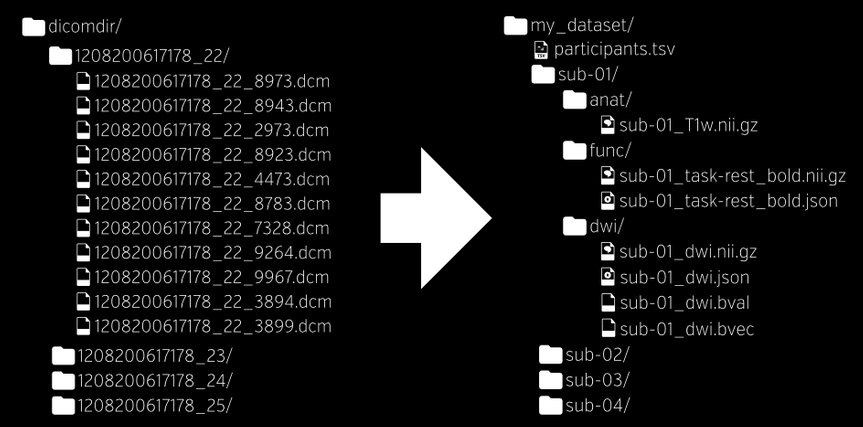
\includegraphics[width=.45\linewidth]{./figures/bids.png}
    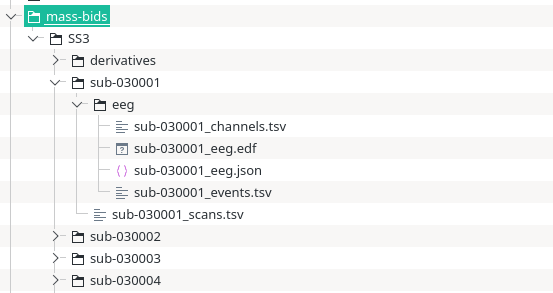
\includegraphics[width=.45\linewidth]{./figures/mass-bids.png}
    \caption{BIDS standard} 
\end{figure}
\begin{itemize}
    \item Neuroimaging data is often complicated to arrange
    \begin{itemize}
        \item Comes from various experiments / medical examinations
        \item Outputs multiple files for a single patient
        \item Little consensus about how to organise files
    \end{itemize}
    \item BIDS standard proposes a way to organise this type of data
    \begin{itemize}
        \item BIDS = Brain Imaging Data Structure \footfullcite{bids, mne-bids, bids-eeg}
        \item subject $>$ session $>$ type / experiment
        \item Compatible with existing software
        \item Captures metadata
    \end{itemize}
\end{itemize}
\end{frame}

\section{Methods}

\subsection{Main steps, code structure}
\begin{frame}{\subsecname}
\begin{columns}
\column{.5\linewidth}
\textbf{Main steps for running our experiment:}
\begin{enumerate}
    \item Loading the datasets
    \item Preprocessing the raw signals and extracting the 30s windows from events
    \item Splitting the dataset into training, validations and testing sets
    \item Creating / loading our model, training and testing
    \item Visualising the results
\end{enumerate}
\column{.5\linewidth}
\textbf{Code structure}, inspired by the \texttt{braindecode}\footfullcite{braindecode} library
\begin{itemize}
    \item \texttt{datasets} to load the datasets that were previously converted to BIDS
    \item \texttt{datautil} to take care of splitting the datasets
    \item \texttt{models} to load and save our models
    \item \texttt{visualisation} for visualising results and the 30s windows
\end{itemize}
\end{columns}
\end{frame}


\subsection{Description of the model}
\begin{frame}{\subsecname}
\begin{itemize}
    \item General feature extractor, denoted by $Z: \mathbb{R}^{C \times T} \rightarrow \mathbb{R}^D$, where $C$ is the number of input channels, $T$ is the number of time steps and $D$ is the size of the estimated feature space
    \item \textbf{Linear spatial filtering}: to estimate virtual channels
    \item \textbf{Convolutional layers}: to capture spectral features
    \item \textbf{Separate pipelines}: to handle several modalities at the same time
    \item Performs \textbf{temporal} sleep staging, that is, takes into account the temporal context of the sample of interest to predict a label
\end{itemize}
\fig{b}{0.8\linewidth}{./figures/model/scheme.png}{Network general architecture}{fig:pipeline}
\end{frame}

\begin{frame}{\subsecname}
\fig{ht!}{.7\linewidth}{./figures/model/model-chambon.png}{Schematic representation of the sleep staging model's architecture}{fig:schema_chambon}
\fig{!ht}{0.5\linewidth}{./figures/model/temporal_scheme.png}{Schematic representation of the time distributed multivariate network}{fig:temporal_context}
\end{frame}

\subsection{Pre-processing, training}
\begin{frame}{\subsecname}
\begin{columns}
\column{.5\linewidth}
\textbf{Preprocessing steps}, using \texttt{mne-python} \footfullcite{mne-python}, same steps as Chambon et al.
\begin{itemize}
    \item Low-pass filtered at 30Hz: to mitigate the impact of higher frequency noise
    \item Downsampled to 100Hz: SleepPhysionet was sampled at 100Hz
    \item Convert signals from V to $\mu$V: very small amplitude brain waves
    \item Cropped 30 minutes of wake events at the beginning and the end of the night
    \item Divided our signal in 30s samples (windows) corresponding to one specific sleep stage
    \item Standardised the windows (zero mean, unit variance): cope for the varying recording conditions
\end{itemize}
\column{.5\linewidth}
\textbf{Training specification}
\begin{itemize}
    \item Implemented with \texttt{PyTorch}
    \item 60 subjects for each experiment, splitted using stratified cross-validation: roughly 60\% of events in training set, 20\% in validation set and 20\% in testing set
    \item Weights initialised with a normal distribution ($\mu = 0$, $\sigma = 0.1$)
    \item Loss function: categorical cross entropy
    \item Optimizer: AdamOptimizer
    \item Minimisation: stochastic gradient descent, learning rate $\texttt{lr} = 5\times10^{-4}$, batch size 8, 10 training epochs
\end{itemize}
\centering
\includegraphics[width=.5\textwidth]{./figures/mne.png}
\end{columns}
\end{frame}


\section{Results and Discussion}
\subsection{Typical results for our experiment}
\begin{frame}{\subsecname}
\begin{columns}
\column{.5\linewidth}
\fig{h}{\linewidth}{./figures/metrics/conf_mat.png}{Confusion matrix for MASS dataset}{fig:conf_mat}
\column{.5\linewidth}
\fig{h}{\linewidth}{./figures/metrics/class_report.png}{Classification report for MASS dataset}{fig:class_report}
\end{columns}
\end{frame}

\subsection{Results of our main experiment and Discussion}
\begin{frame}{\subsecname}
\begin{table}[h]
    \centering
    \tiny
    \begin{tabular}{|c||c|c|}
    \hline
    \diagbox{Training set}{Testing set} & MASS              & SleepPhysionet    \\ 
    \hline \hline
    MASS              & \textbf{0.802}    & \textbf{0.487}    \\ 
    \hline
    SleepPhysionet     & \textbf{0.560}    & \textbf{0.634}        \\  
    \hline
    \end{tabular}
    \begin{tabular}{|c||c|c|}
    \hline
    \diagbox{Training set}{Testing set} & MASS              & Clinical          \\ 
    \hline \hline
    MASS               & \textbf{0.817}    & \textbf{0.390}    \\ 
    \hline
    Clinical           & \textbf{0.530}    & \textbf{0.635}    \\  
    \hline
    \end{tabular}
    \caption{Balanced accuracy for main experiment}
    \label{tab:scores}
\end{table}
\begin{itemize}
    \item Clinical-Clinical and SleepPhysionet-SleepPhysionet lower than expected
    \begin{itemize}
        \item Pre-processing steps
        \item Model initially benchmarked using MASS, model biased towards MASS?
        \item Hyperparameters are not optimal
    \end{itemize}
    \item Model transfers better from SleepPhysionet/Clinical to MASS than from MASS to SleepPhysionet/Clinical
    \begin{itemize}
        \item Specificity in the MASS dataset?
    \end{itemize}
    \item Domain adaptation remains one of the big challenges of sleep scoring algorithms
    \item Increasing number of EEG channels and adding EOG and EMG data greatly improves performance
\end{itemize}
\end{frame}

\subsection{Limitations and Further Works}
\begin{frame}{\subsecname}
\begin{itemize}
    \item SleepPhysionet scored according to the Rechtschaffen and Kales guidelines, MASS and Clinical scored according to the AASM guidelines
    \begin{itemize}
        \item N4 sleep stage
        \item Transition rules
    \end{itemize}
    \item Tune hyperparameters and improve the model’s architecture to get better performance on Clinical and SleepPhysionet
    \item Core differences in terms of data
    \begin{itemize}
        \item Clinical datasets are in general more difficult to work with
    \end{itemize}
\end{itemize}
\end{frame}

\section{Conclusion}

\subsection{Perspectives}
\begin{frame}{\subsecname}
\centering
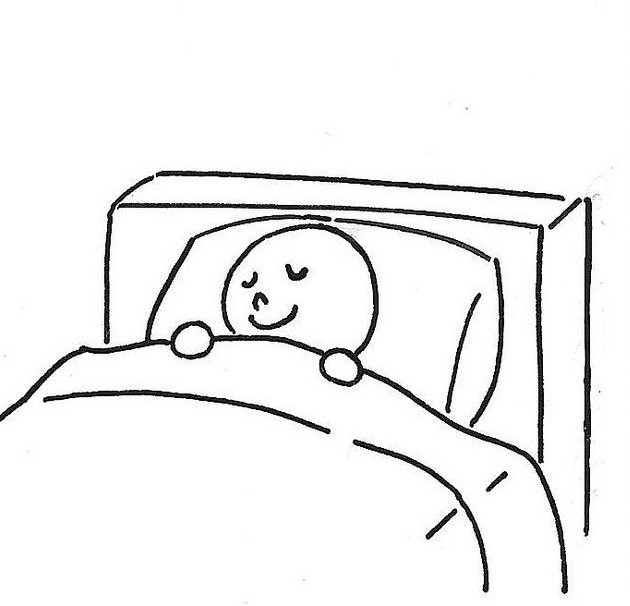
\includegraphics[width=.75\linewidth]{./figures/sleep2.png}
\end{frame}

\subsection[Acknowledge-ments]{Acknowledgements}
\begin{frame}{\subsecname}
\centering

\includegraphics[width=.75\linewidth]{./figures/thanks.jpg}
\end{frame}

\section*{Annex}
\begin{frame}{\secname}

\begin{table}[!ht]
    \centering
    \begin{tabular}{c|c|c|}
    \cline{2-3}
    & MASS              & SleepPhysionet    \\ 
    \hline
    \multicolumn{1}{|c|}{\rotatebox{90}{\centering MASS}}   & 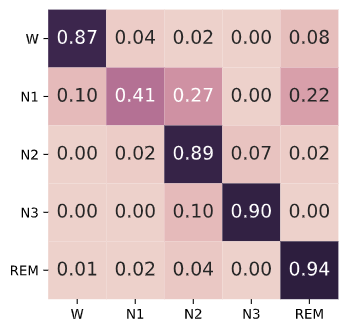
\includegraphics[width=0.3\linewidth]{./figures/confusion_matrix/mass-mass-4ch.png}    & 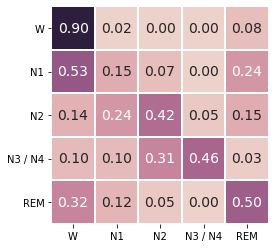
\includegraphics[width=0.3\linewidth]{./figures/confusion_matrix/mass-sp.png}     \\ 
    \hline
    \multicolumn{1}{|c|}{\rotatebox{90}{\centering SleepPhysionet}} & 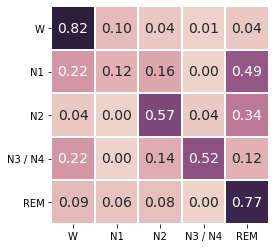
\includegraphics[width=0.3\linewidth]{./figures/confusion_matrix/sp-mass.png}    & 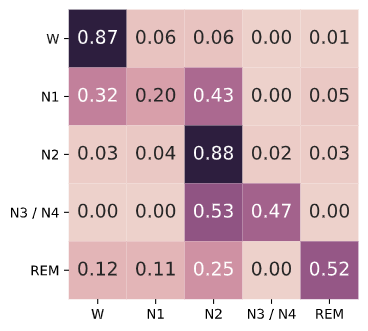
\includegraphics[width=0.3\linewidth]{./figures/confusion_matrix/sp-sp.png}        \\  
    \hline
    \end{tabular}
    \caption{Table of confusion matrices, comparing the datasets MASS and SleepPhysionet}
    \label{tab:conf_mat_sp}
\end{table}
\end{frame}

\begin{frame}
\begin{table}[!ht]
    \centering
    \begin{tabular}{c|c|c|}
    \cline{2-3}
    & MASS              & SleepPhysionet    \\ 
    \hline
    \multicolumn{1}{|c|}{\rotatebox{90}{\centering MASS}}   & 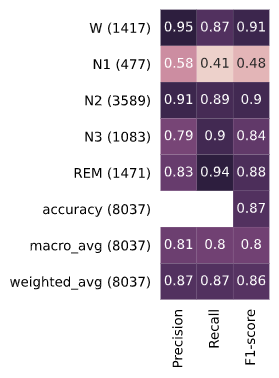
\includegraphics[width=0.25\linewidth]{./figures/classification_report/mass-mass-4ch.png}    & 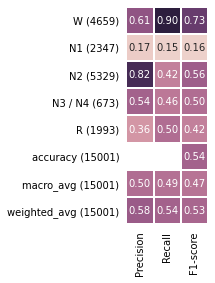
\includegraphics[width=0.25\linewidth]{./figures/classification_report/mass-sp.png}     \\ 
    \hline
    \multicolumn{1}{|c|}{\rotatebox{90}{\centering SleepPhysionet}} & 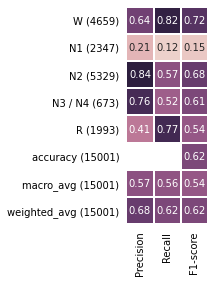
\includegraphics[width=0.25\linewidth]{./figures/classification_report/sp-mass.png}    & 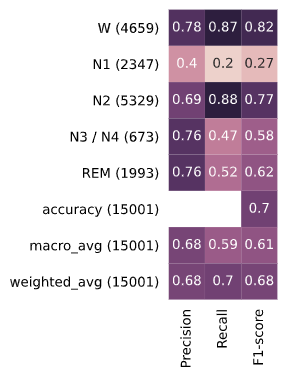
\includegraphics[width=0.25\linewidth]{./figures/classification_report/sp-sp.png}        \\  
    \hline
    \end{tabular}
    \caption{Table of classification reports, comparing the datasets MASS and SleepPhysionet}
    \label{tab:class_report_sp}
\end{table}
\end{frame}

\begin{frame}
\begin{table}[ht!]
    \centering
    \begin{tabular}{c|c|c|}
    \cline{2-3}
    & MASS              & Clinical    \\ 
    \hline
    \multicolumn{1}{|c|}{\rotatebox{90}{\centering MASS}}   & 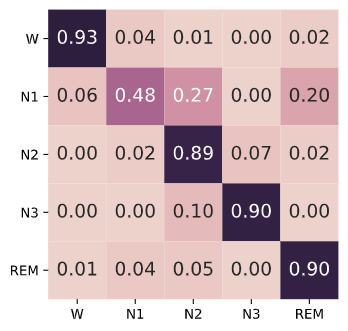
\includegraphics[width=0.3\linewidth]{./figures/confusion_matrix/mass-mass-9ch.png}    & 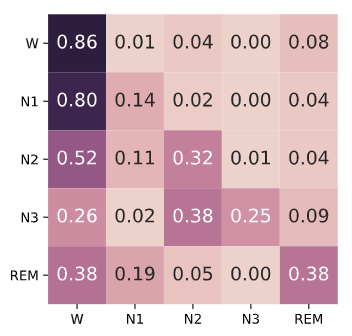
\includegraphics[width=0.3\linewidth]{./figures/confusion_matrix/mass-clin.png}     \\ 
    \hline
    \multicolumn{1}{|c|}{\rotatebox{90}{\centering Clinical}} & 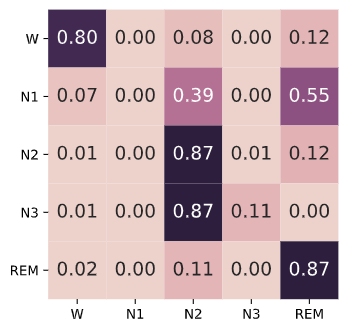
\includegraphics[width=0.3\linewidth]{./figures/confusion_matrix/clin-mass.png}    & 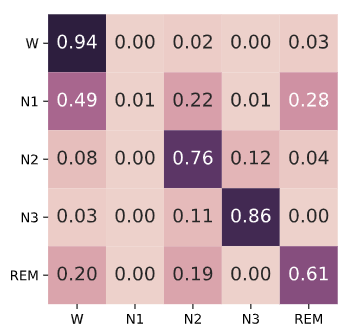
\includegraphics[width=0.3\linewidth]{./figures/confusion_matrix/clin-clin.png}        \\  
    \hline
    \end{tabular}
    \caption{Table of confusion matrices, comparing the datasets MASS and Clinical}
    \label{tab:conf_mat_clin}
\end{table}
\end{frame}

\begin{frame}
\begin{table}[ht!]
    \centering
    \begin{tabular}{c|c|c|}
    \cline{2-3}
    & MASS              & Clinical    \\ 
    \hline
    \multicolumn{1}{|c|}{\rotatebox{90}{\centering MASS}}   & 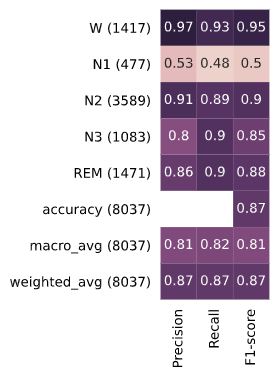
\includegraphics[width=0.25\linewidth]{./figures/classification_report/mass-mass-9ch.png}    & 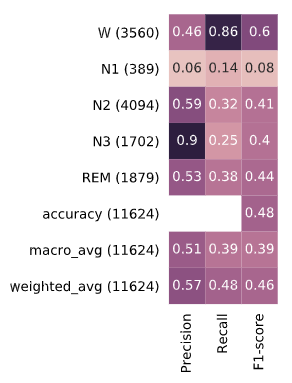
\includegraphics[width=0.25\linewidth]{./figures/classification_report/mass-clin.png}     \\ 
    \hline
    \multicolumn{1}{|c|}{\rotatebox{90}{\centering Clinical}} & 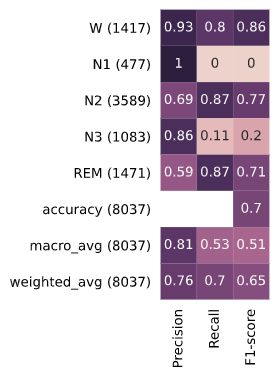
\includegraphics[width=0.25\linewidth]{./figures/classification_report/clin-mass.png}    & 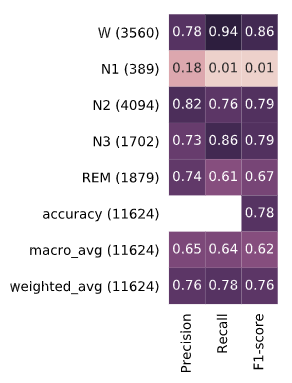
\includegraphics[width=0.25\linewidth]{./figures/classification_report/clin-clin.png}        \\  
    \hline
    \end{tabular}
    \caption{Table of classification reports, comparing the datasets MASS and Clinical}
    \label{tab:class_rep_clin}
\end{table}
\end{frame}

\end{document}
